% !TEX TS-program = pdflatex
% !TEX encoding = UTF-8 Unicode

% This is a simple template for a LaTeX document using the "article" class.
% See "book", "report", "letter" for other types of document.

\documentclass[11pt]{article} % use larger type; default would be 10pt

\usepackage[utf8]{inputenc} % set input encoding (not needed with XeLaTeX)

%%% Examples of Article customizations
% These packages are optional, depending whether you want the features they provide.
% See the LaTeX Companion or other references for full information.

%%% PAGE DIMENSIONS
\usepackage{geometry} % to change the page dimensions
\geometry{a4paper} % or letterpaper (US) or a5paper or....
% \geometry{margin=2in} % for example, change the margins to 2 inches all round
% \geometry{landscape} % set up the page for landscape
%   read geometry.pdf for detailed page layout information

\usepackage{graphicx} % support the \includegraphics command and options

% \usepackage[parfill]{parskip} % Activate to begin paragraphs with an empty line rather than an indent

%%% PACKAGES
\usepackage{booktabs} % for much better looking tables
\usepackage{array} % for better arrays (eg matrices) in maths
%\usepackage{paralist} % very flexible & customisable lists (eg. enumerate/itemize, etc.)
\usepackage{verbatim} % adds environment for commenting out blocks of text & for better verbatim
\usepackage{subfig} % make it possible to include more than one captioned figure/table in a single float
% These packages are all incorporated in the memoir class to one degree or another...

%%% HEADERS & FOOTERS
\usepackage{fancyhdr} % This should be set AFTER setting up the page geometry
\pagestyle{fancy} % options: empty , plain , fancy
\renewcommand{\headrulewidth}{0pt} % customise the layout...
\lhead{}\chead{}\rhead{}
\lfoot{}\cfoot{\thepage}\rfoot{}

%%% SECTION TITLE APPEARANCE
\usepackage{sectsty}
\allsectionsfont{\sffamily\mdseries\upshape} % (See the fntguide.pdf for font help)
% (This matches ConTeXt defaults)

%%% ToC (table of contents) APPEARANCE
\usepackage[nottoc,notlof,notlot]{tocbibind} % Put the bibliography in the ToC
\usepackage[titles,subfigure]{tocloft} % Alter the style of the Table of Contents
\renewcommand{\cftsecfont}{\rmfamily\mdseries\upshape}
\renewcommand{\cftsecpagefont}{\rmfamily\mdseries\upshape} % No bold!

%%% END Article customizations

\usepackage[spanish]{babel}
\usepackage{listings} 
%%% The "real" document content comes below...

\title{Investigación de Lenguajes - SCHEME}
%\date{} % Activate to display a given date or no date (if empty),
         % otherwise the current date is printed 

\begin{document}
\maketitle
%\tableofcontents % No hace falta un TOC en un artículo corto
\begin{itemize}
\item Adrian Aguilar
\item Edinson Sanchez
\item Kevin Filella
\end{itemize}

\section{Introducción}
asdf

\section{Características}
\section{Historia}
\subsection{Carl Hewitt y el proyecto Planner}

En 1971, Gerald Jay Sussman, Drew McDermott y Eugene Charniak desarrollaron un sistema llamado Micro-Planner, una parcial e insatisfactoria implementación de Planner. Sussman y Carl Hewitt trabajaron, junto con otros, en Muddle (luego MDL), una extensión de Lisp que formo un componente del proyecto Planner de Hewitt. En 1972, Sussman y McDermott desarrollaron un lenguaje basado en Lisp llamado Conniver.

En noviembre de 1972, Hewitt y sus estudiantes en el MIT desarrollaron el modelo Actor en computación, el cual fue propuesto como una solución a los problemas con Planner. Steele y Sussman luego decidieron implementar una versión del modelo Actor en MacLisp. Comenzaron a desarrollar mecanismos para crear actores y enviar mensajes.

\subsection{Implementacion del modelo Actor y el nacimiento de Scheme}

Sussman y Guy L. Steele luego implementaron el modelo Actor en el cálculo lambda, llamando a su sistema de modelación: Schemer. Este nombre fue luego reducido a 'Scheme' ya que hicieron uso del sistema operativo ITS, que limitaba los nombres de fichero a seis caracteres. Luego, ambos concluyeron que los Actores y los Closures eran, para propósitos de sus investigaciones, un concepto idéntico y procedieron a eliminar el código redundante. Luego de la eliminación, se dieron cuenta que habían creado un pequeño, y muy capaz, dialecto de Lisp.

Hewitt estuvo escéptico de las capacidades del cálculo lambda como base de la programación y dijo, "La actual situación es que el cálculo lambda es capaz de expresar ciertos tipos de estructuras de control paralelo y secuencial, pero, en general, no es capaz de expresar la concurrencia que expresa el modelo Actor. Por otro lado, el modelo Actor es capaz de expresar todo lo del cálculo lambda, y mas." Hewitt también ha sido fuerte en las criticas sobre Scheme en base a su falta de manejo de excepciones y su dependencia a lo que se llaman continuation functions.

\subsection{Publicación y Estandarización}

Scheme es un lenguaje de programación que enfatiza la aplicación de funciones, o lenguaje funcional, que tiene sus raíces en el lenguaje de programación Lisp, siendo un dialecto de este. Scheme tuvo sus inicios en el periodo de 1975 hasta 1980, cuando Guy L. Steele y Gerald Jay Sussman, del MIT AI Lab, publicaron nueve artículos llamados Lambda Papers durante este tiempo.

Aunque una de las características mas importantes de destacar sobre Scheme es el minimalismo, Sussman y Steele expresaron que esta no fue una meta intencional durante su creación. "Nosotros en realidad estábamos tratando de construir algo complicado y rebuscado, favorablemente, habíamos creado algo que, además de cumplir con todas nuestras metas, era mucho más simple de lo intencionado... Nos dimos cuenta que el cálculo lambda puede servir como la base de un poderoso lenguaje de programación." (Gerald Jay Sussman y Guy L. Steele, Jr. (Diciembre 1998). "The First Report on Scheme Revisited").

Scheme tiene un estándar oficial de la IEEE y un estándar de facto llamado Revised n-th Report on the Algorithmic Language Scheme (comunmente abreviado RnRS). El estándar mas implementado hasta la fecha es el R5RS de 1998, y el nuevo estándar, R6RS, fue ratificado el 2007.
\section{Tutorial de Instalación}
\subsection{Debemos ir al siguiente link (http://www.gnu.org/software/mit-scheme/) y descargar el paquete de instalación del lenguaje SCHEME correspondiente al sistema operativo en la q se va a trabajar, en este caso yo instalare el paquete de Windows 7.
lo elegimos e inmediatamente comenzara la descarga del paquete de instalación}
\begin{center}
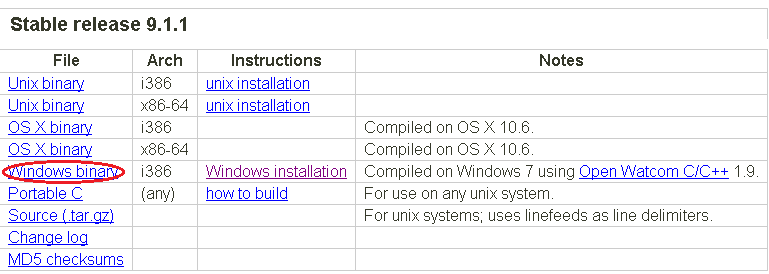
\includegraphics[width=12cm]{1.png}
\end{center}

\subsection{Ejecutamos el paquete de instalación de SCHEME y aparecerá la siguiente ventana donde le damos en NEXT}
\begin{center}
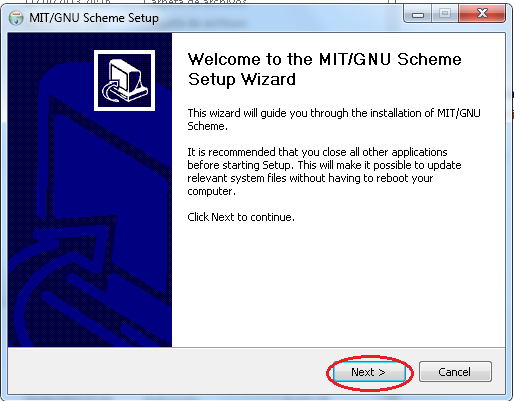
\includegraphics[width=12cm]{2.png}
\end{center}

\subsection{Ahora nos aparecerá una nueva ventana donde estarán los términos de licencia del programa, si está de acuerdo le da clic en  I AGREE, caso contrario atrás o cancelar}
\begin{center}
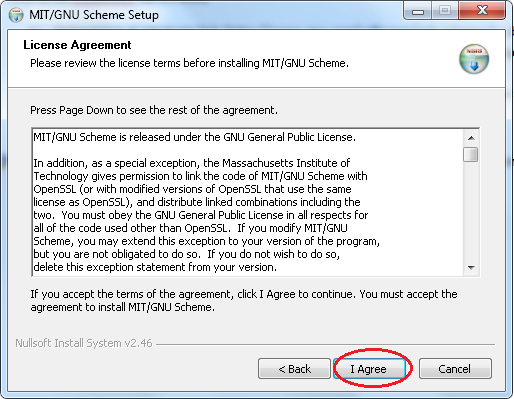
\includegraphics[width=12cm]{3.png}
\end{center}

\subsection{Nos aparecerá otra ventana donde debemos ingresar una dirección e el disco duro donde queremos q el programa se instale, si quiere puede dejar la dirección que se encuentra escrita por defecto y le da clic en NEXT}
\begin{center}
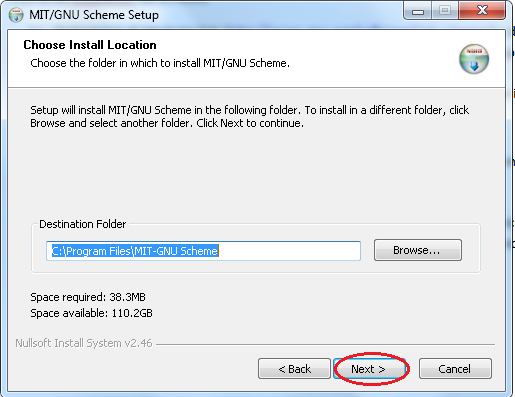
\includegraphics[width=12cm]{4.png}
\end{center}

\subsection{Aparecerá una nueva ventana donde podemos cambiar el nombre a la carpeta donde se va a instalar el programa, si quieren pueden dejar el nombre que se encuentra por defecto y dar clic en  INSTALL }
\begin{center}
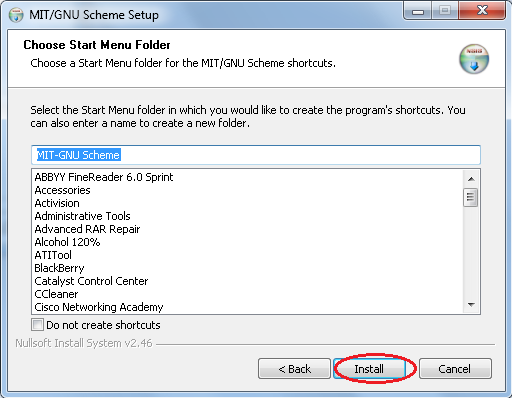
\includegraphics[width=12cm]{5.png}
\end{center}

\subsection{Comenzara a instalarse el programa hasta que la barra llegue al 100 y aparecerá una nueva ventana donde le damos clic en FINISH para confirmar que el programa se ha instalado correctamente}
\begin{center}
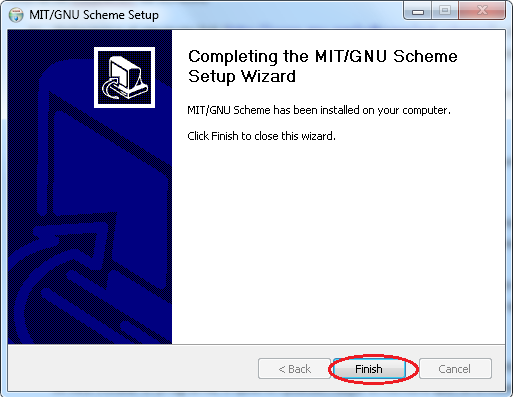
\includegraphics[width=12cm]{6.png}
\end{center}

\subsection{Ahora vemos en nuestro escritorio y nos va a aparecer un nuevo icono que le pertenece al programa SCHEME recién instalado, le damos doble clic y se abrirá}
\begin{center}
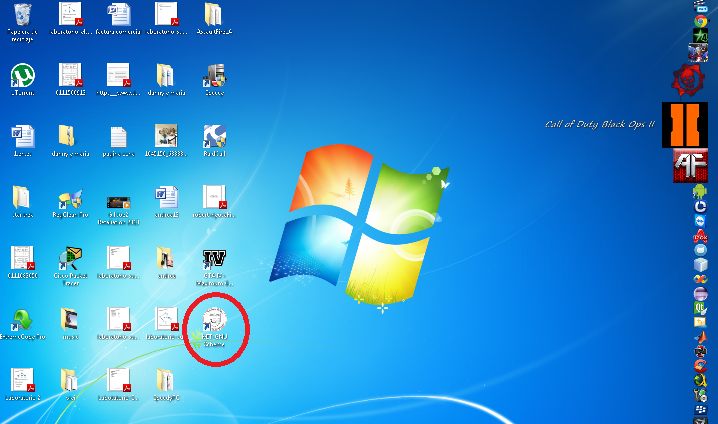
\includegraphics[width=12cm]{7.png}
\end{center}

\subsection{Finalmente tenemos instalado en nuestro ordenador el lenguaje SCHEME listo para trabajar}
\begin{center}
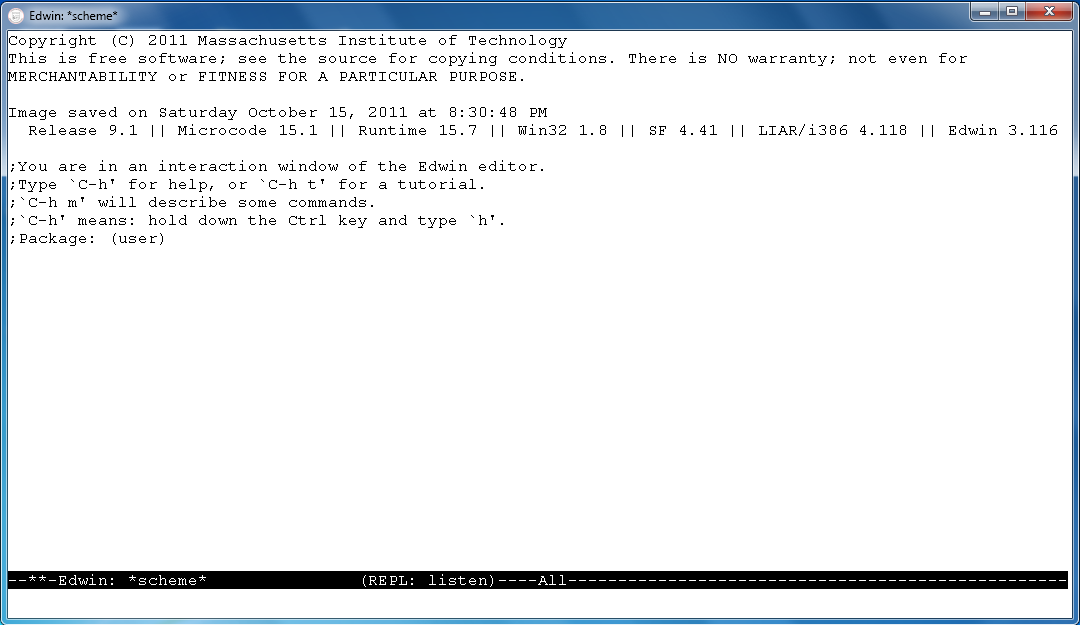
\includegraphics[width=12cm]{8.png}
\end{center}

\section{Hola Mundo y otros Programas Introductorios}

\lstset{language=Pascal}          % Set your language (you can change the language for each code-block optionally)

\begin{lstlisting}[frame=single]  % Start your code-block
for i:=maxint to 0 do
begin
{ do nothing }
end;
Write('Case insensitive ');
Write('Pascal keywords.');
\end{lstlisting}



\end{document}
